\documentclass[a4paper,landscape,hidelinks,14pt]{extarticle}

\usepackage[T2A]{fontenc}
\usepackage[utf8]{inputenc}
\usepackage[russian]{babel}
\usepackage{cmap}

\usepackage{xcolor}

\usepackage{helvet}
\usepackage{pscyr}

\usepackage{multicol}

\usepackage{amssymb,amsfonts,amsmath,mathtext}
\usepackage{cite,enumerate,float}

\usepackage{listings}
\usepackage{tikz}

\graphicspath{{images/}}           % Подключаемые пакеты
../../../templates/presentation/sys/styles.tex             % Пользовательские стили

\begin{document}
../../../templates/magistracy_dissertation_synopsis/sys/names.tex              % Переопределение именований

Объект \( \eta = \alpha + \beta \xi, \alpha = 0 \),
где \( \xi \) и \( \eta \) --- фактические значения входа и выхода,
\( \alpha, \beta \) --- фактические значения параметров.

Наблюдаются вход \( x = \xi + \epsilon \), выход \( y = \eta + \delta \),
так что \( x \) и \( y \) --- наблюдения входа и выхода.
С.к.о. ошибок измерений \( \sigma_x, \sigma_y \).

Значения \( \xi \) выбирались из равномерного в \( [0, 10] \) распределения.
Для получения одной оценки \( ( \alpha, \beta ) \) использовались 100 наблюдений
\( ( x_i, y_i ), i = \overline{1, 100} \). Расчеты расстояний по параметрам и по выходу
велись в узлах сетки значений \( \sigma_x, \sigma_y \) в прямоугольнике
\( [0, 2] \times [0, 2] \) с шагом 0{,}1. В каждом узле сетки вычислялось 100 оценок.

На приведенных ниже графиках приведены следующие зависимости
разности точностей оценок, полученных МНК и методом Пирсона, от
с.к.о. ошибок измерений входной и выходной переменной:
\begin{itemize}
\item параметров (слева);
\item прогнозов наблюдаемых значений выхода (в центре);
\item прогнозов фактических значений выхода (справа).
\end{itemize}

Отрицательные значения свидетельствуют о том, что при данных значениях
c.к.о. ошибок измерений МНК дает более точные значения, чем метод Пирсона;
положительные --- наоборот.

Анализ приведенных зависимостей показывает, что:
\begin{enumerate}
\item Точность оценок параметров зависит от коэффициента усиления системы и
  значений с.к.о. ошибок измерений входных и выходных переменных.
  При больших значениях коэффициента усиления и с.к.о. ошибок измерения
  метод Пирсона дает более точные оценки, чем классическая линейная регрессия.
  В прочих условиях оценки, полученные классическим методом, имеют большую точность.
  Для того, чтобы решить, какой метод даёт более точные оценки параметров,
  предлагаем использовать следующее эмпирическое правило:
  <<Если \( \sigma_{\delta} > (0{,}7 + |\beta|) \sigma_{\epsilon} \),
  то классическая регрессия дает более точные оценки параметров>>.
  В противном случае следует предпочесть метод Пирсона.
\item Классическая линейная регрессия дает более точные оценки
  фактических и наблюдаемых выходных значений, чем метод Пирсона,
  во всем рассмотренном диапазоне значений коэффициента усиления системы и
  с.к.о ошибок измерений.
\end{enumerate}

\begin{figure}[h!]
  \centering
  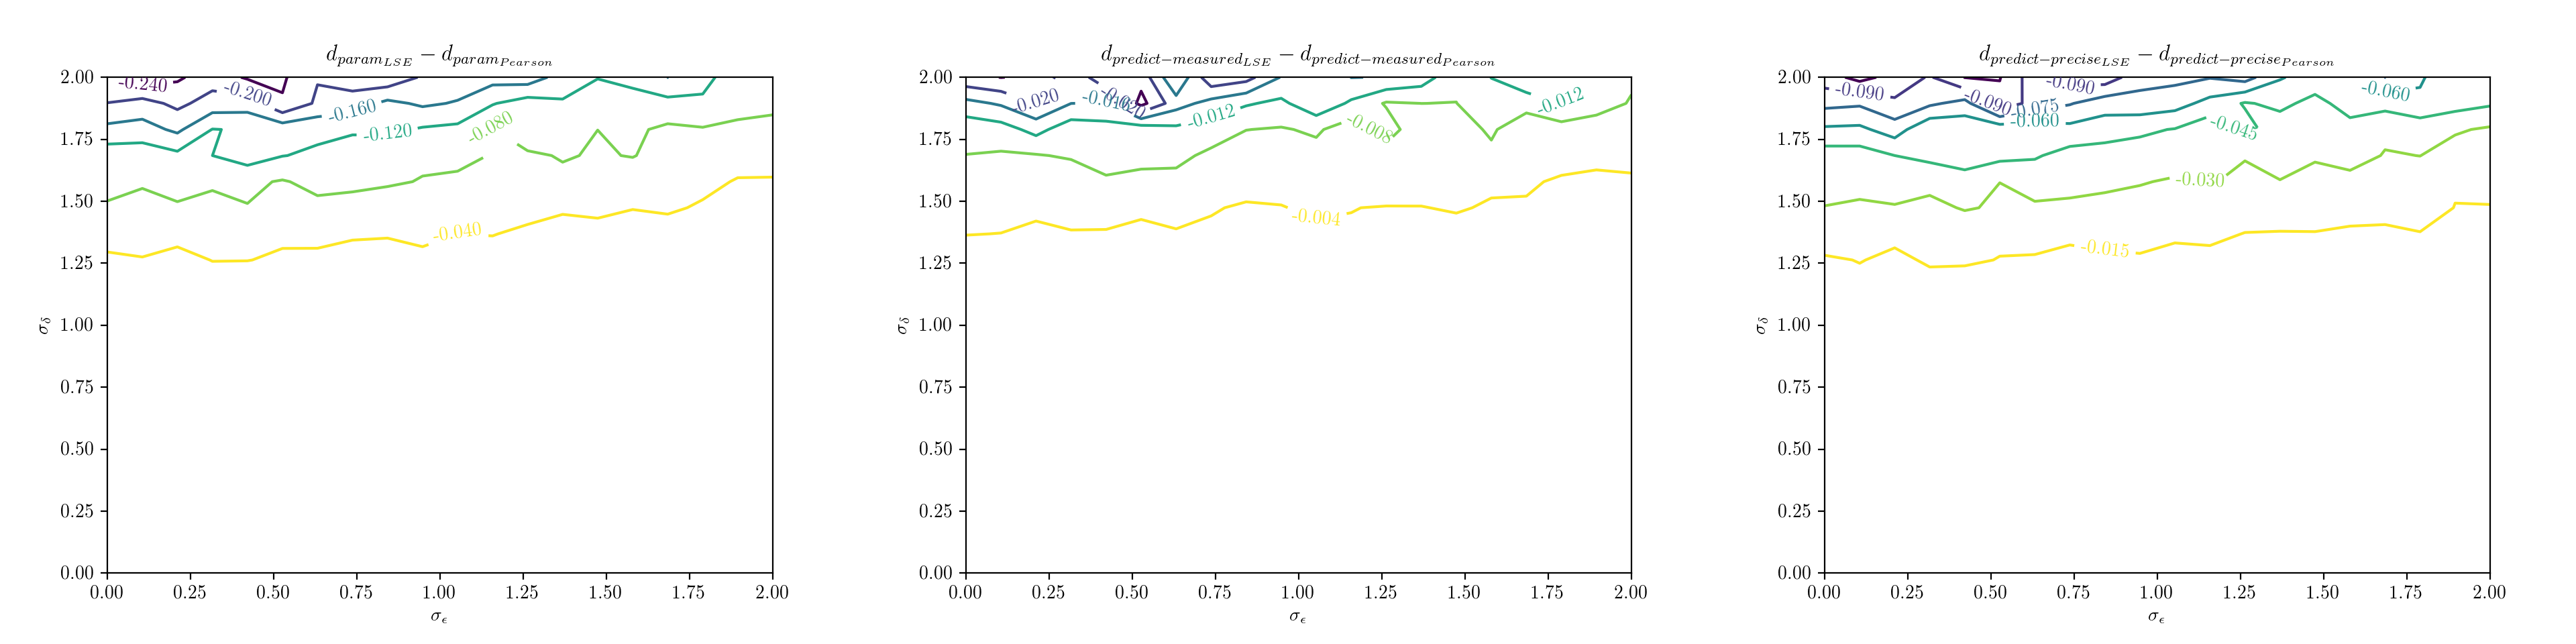
\includegraphics[width=.9\linewidth]{fig/beta-0.png}
  \caption{$ \beta = 0 $}
\end{figure}

\begin{figure}[h!]
  \centering
  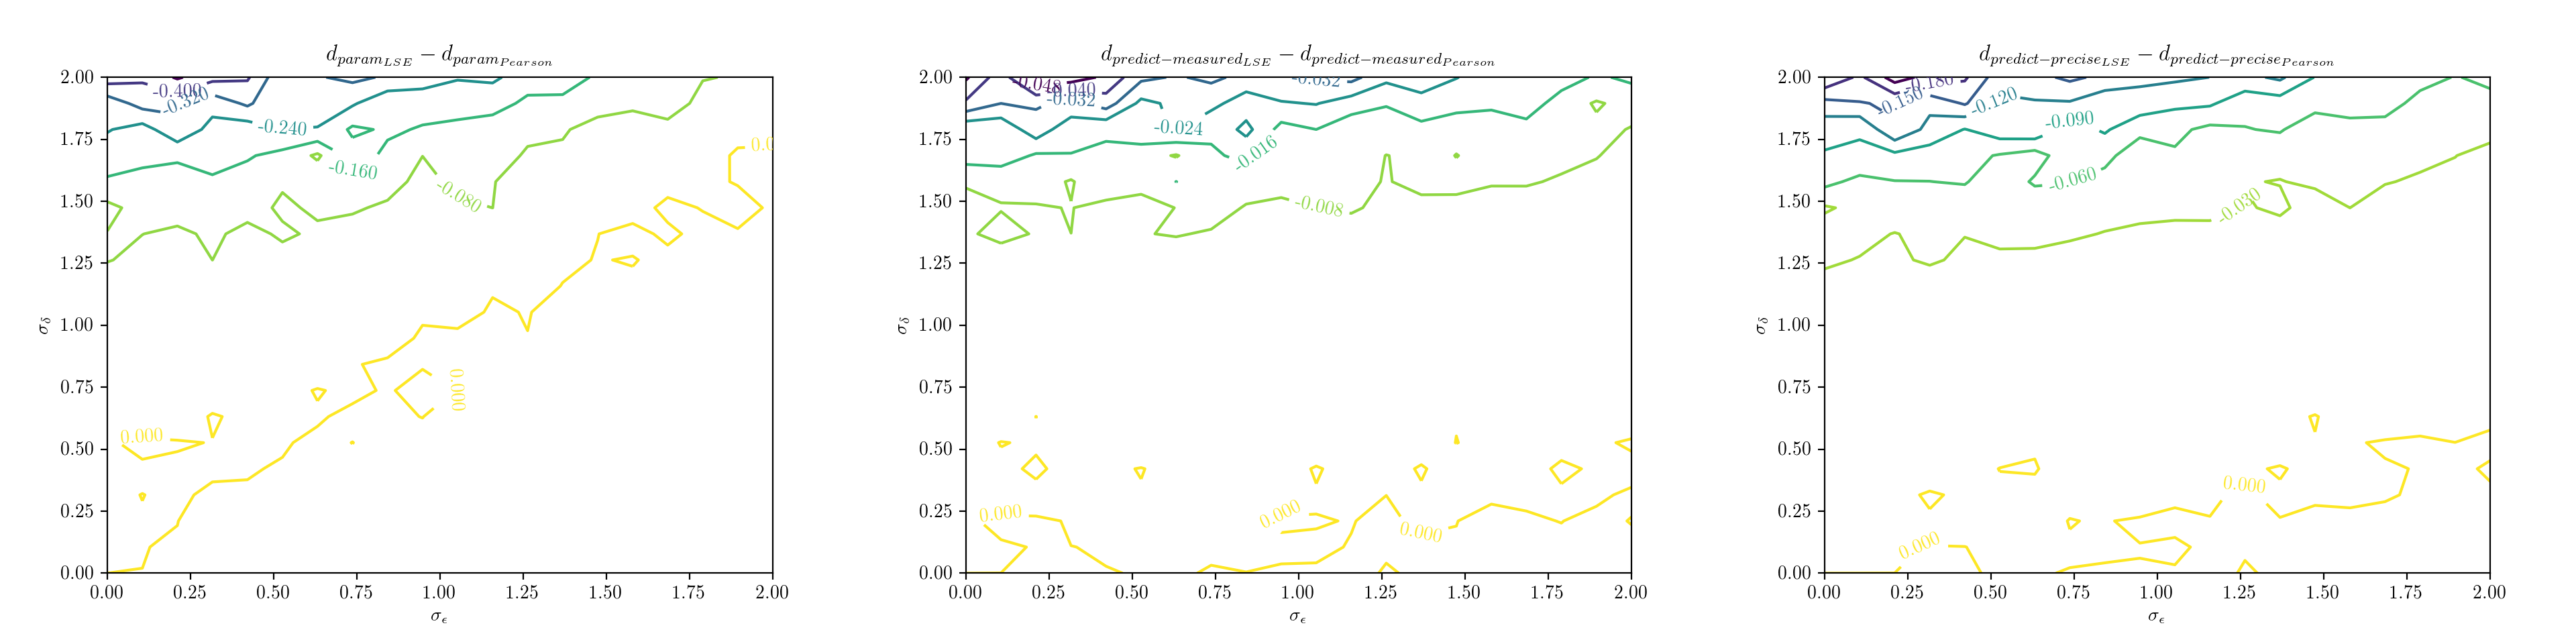
\includegraphics[width=.9\linewidth]{fig/beta-0,125.png}
  \caption{$ \beta = 0.125 $}
\end{figure}

\begin{figure}[h!]
  \centering
  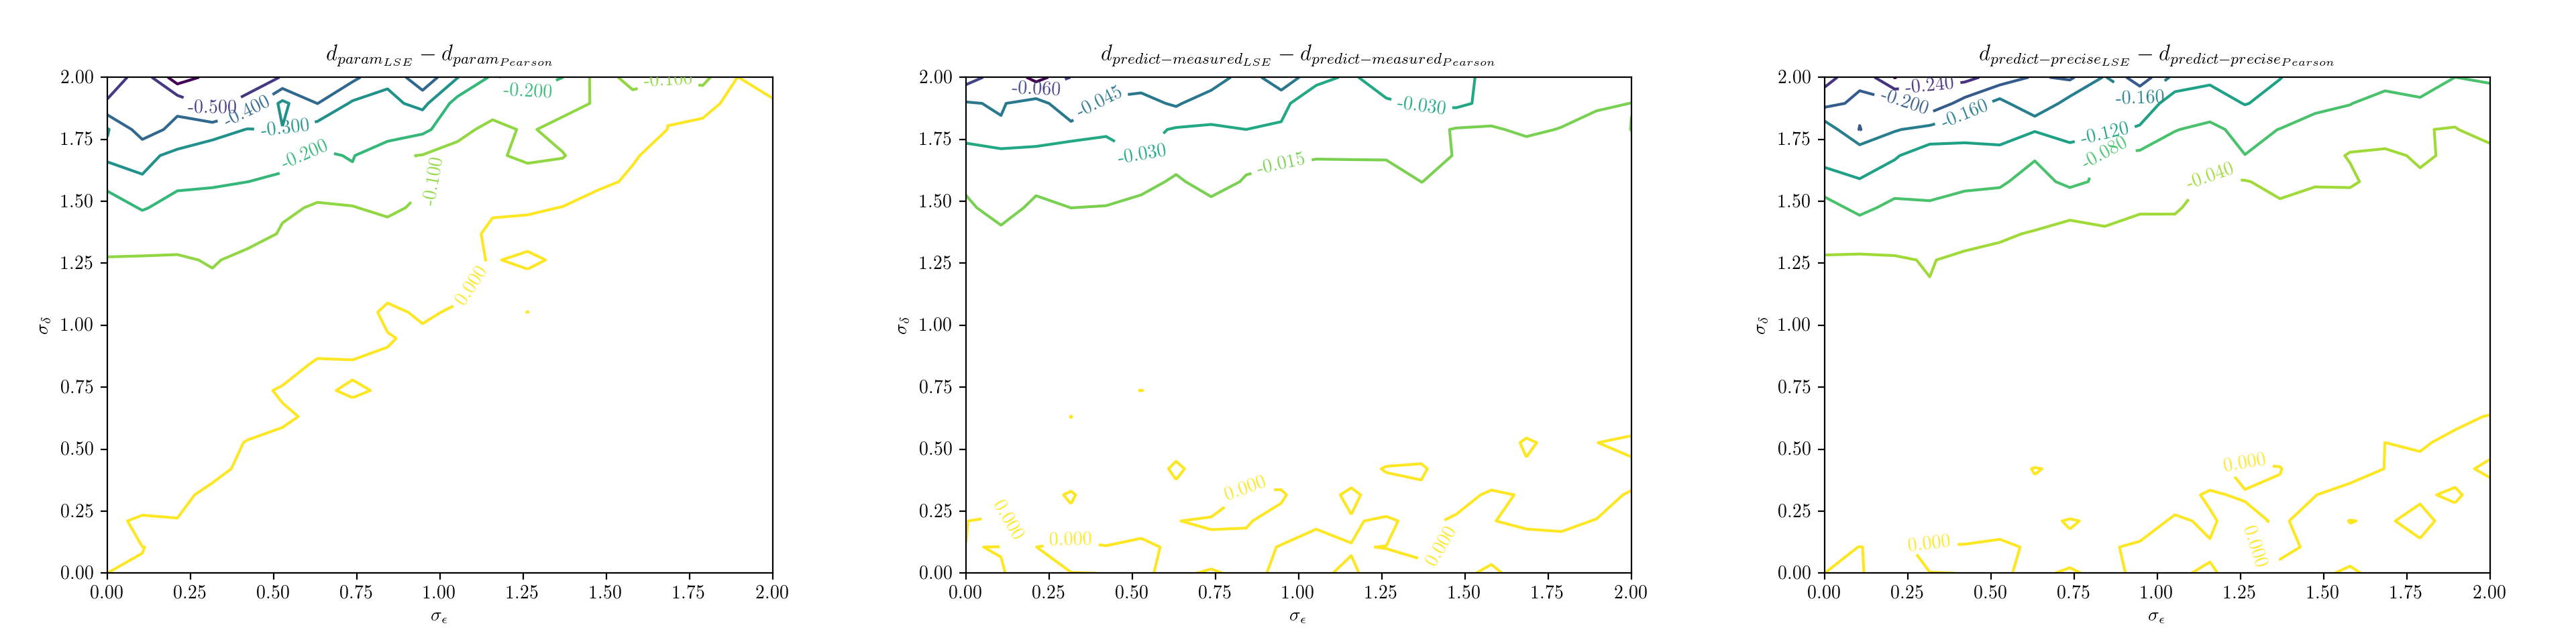
\includegraphics[width=.9\linewidth]{fig/beta-0,2.png}
  \caption{$ \beta = 0.2 $}
\end{figure}

\begin{figure}[h!]
  \centering
  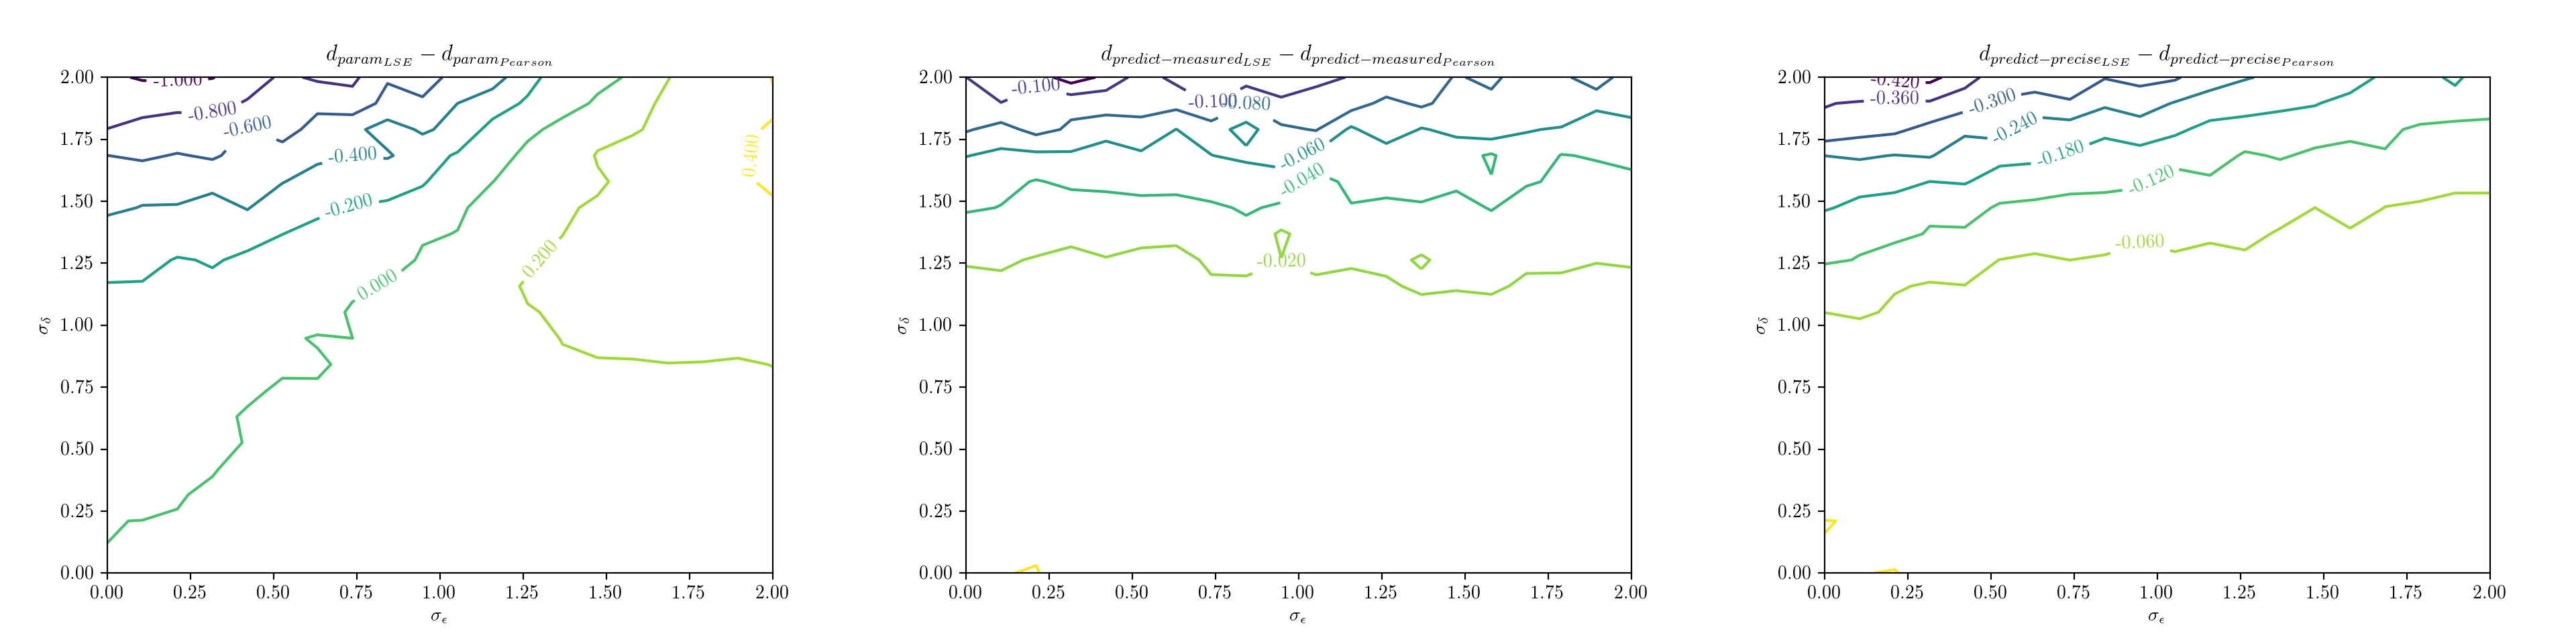
\includegraphics[width=.9\linewidth]{fig/beta-0,5.png}
  \caption{$ \beta = 0.5 $}
\end{figure}

\begin{figure}[h!]
  \centering
  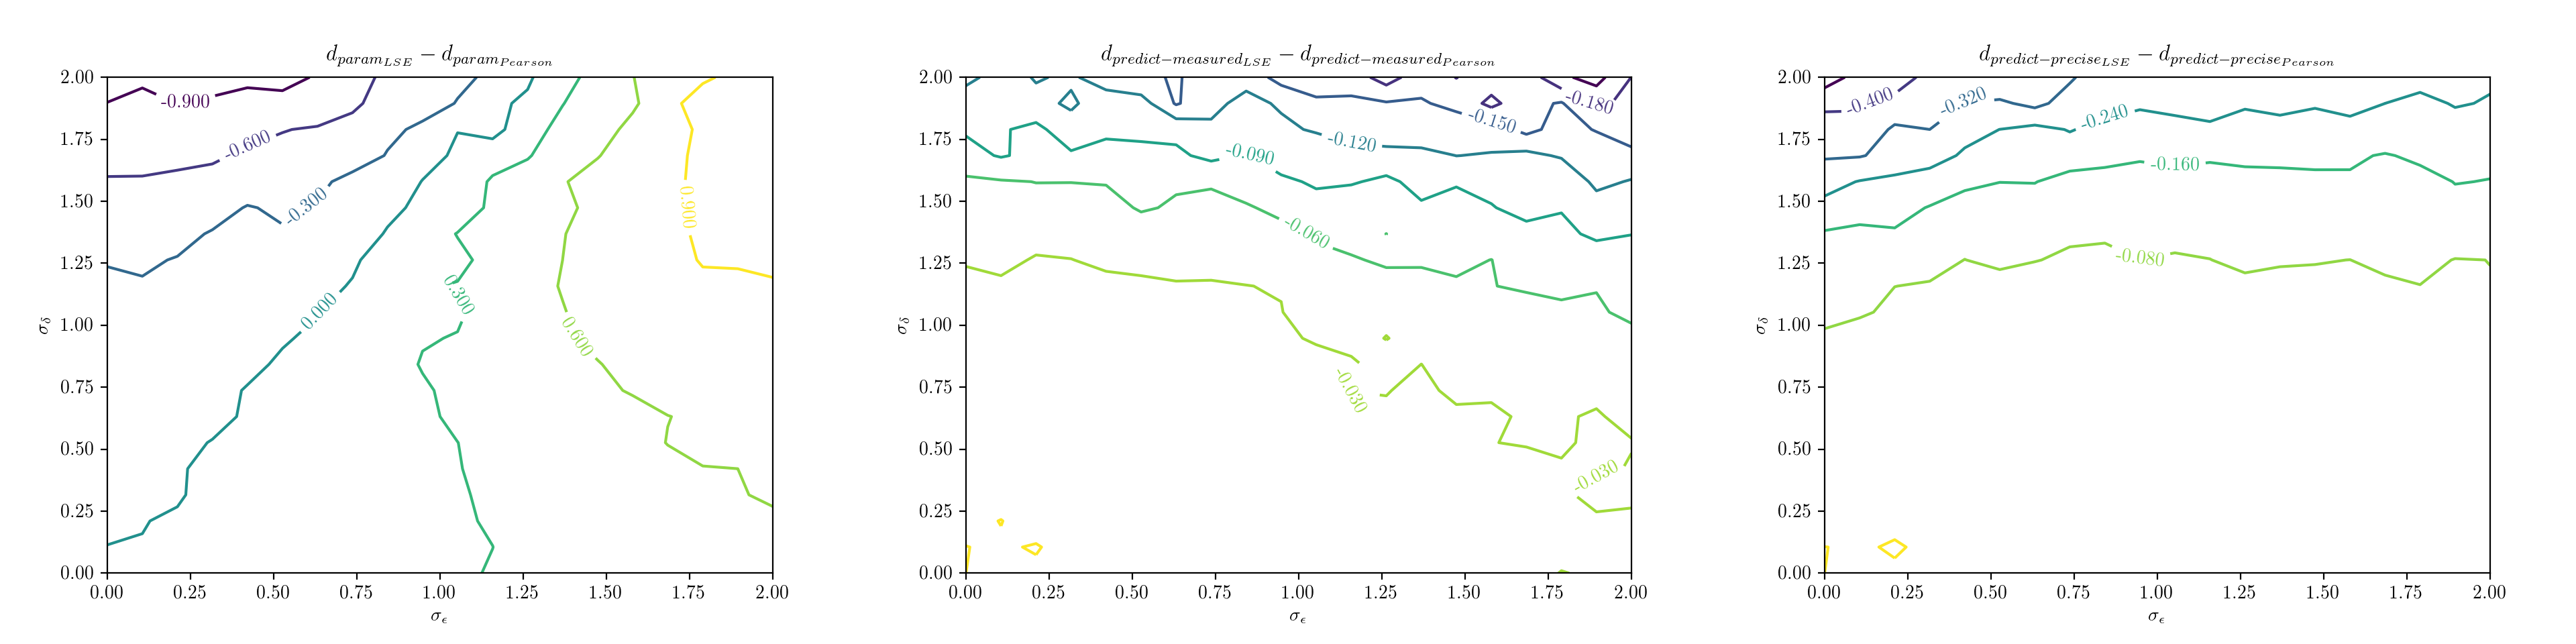
\includegraphics[width=.9\linewidth]{fig/beta-1.png}
  \caption{$ \beta = 1 $}
\end{figure}

\begin{figure}[h!]
  \centering
  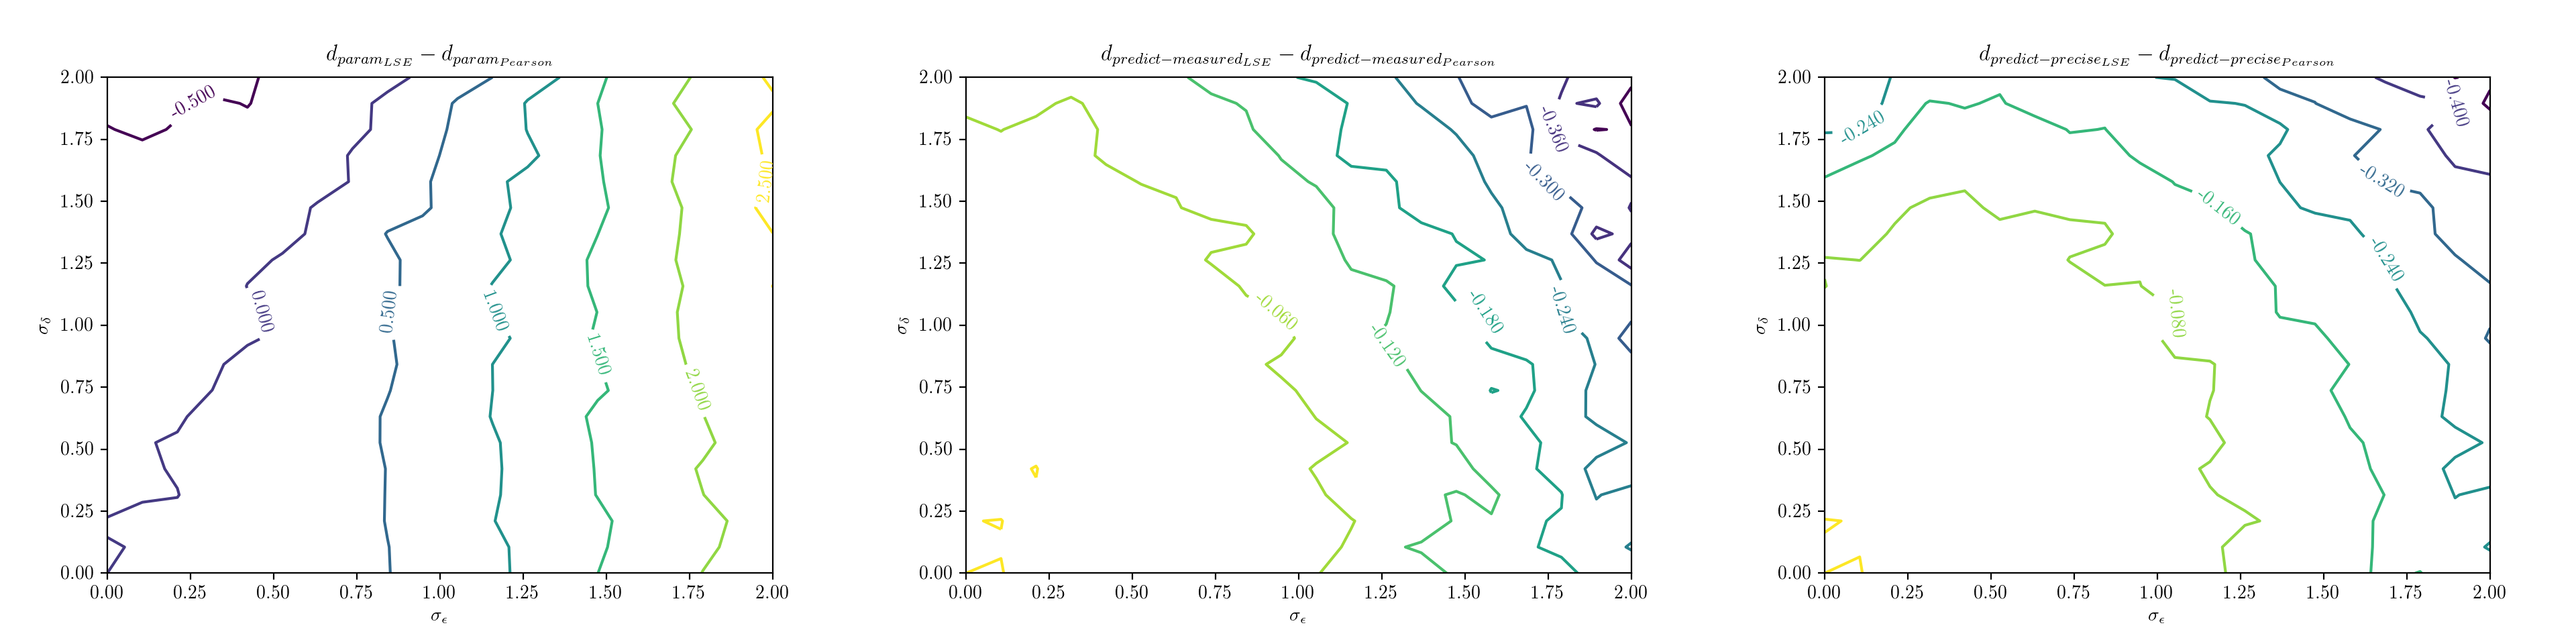
\includegraphics[width=.9\linewidth]{fig/beta-2.png}
  \caption{$ \beta = 2 $}
\end{figure}

\begin{figure}[h!]
  \centering
  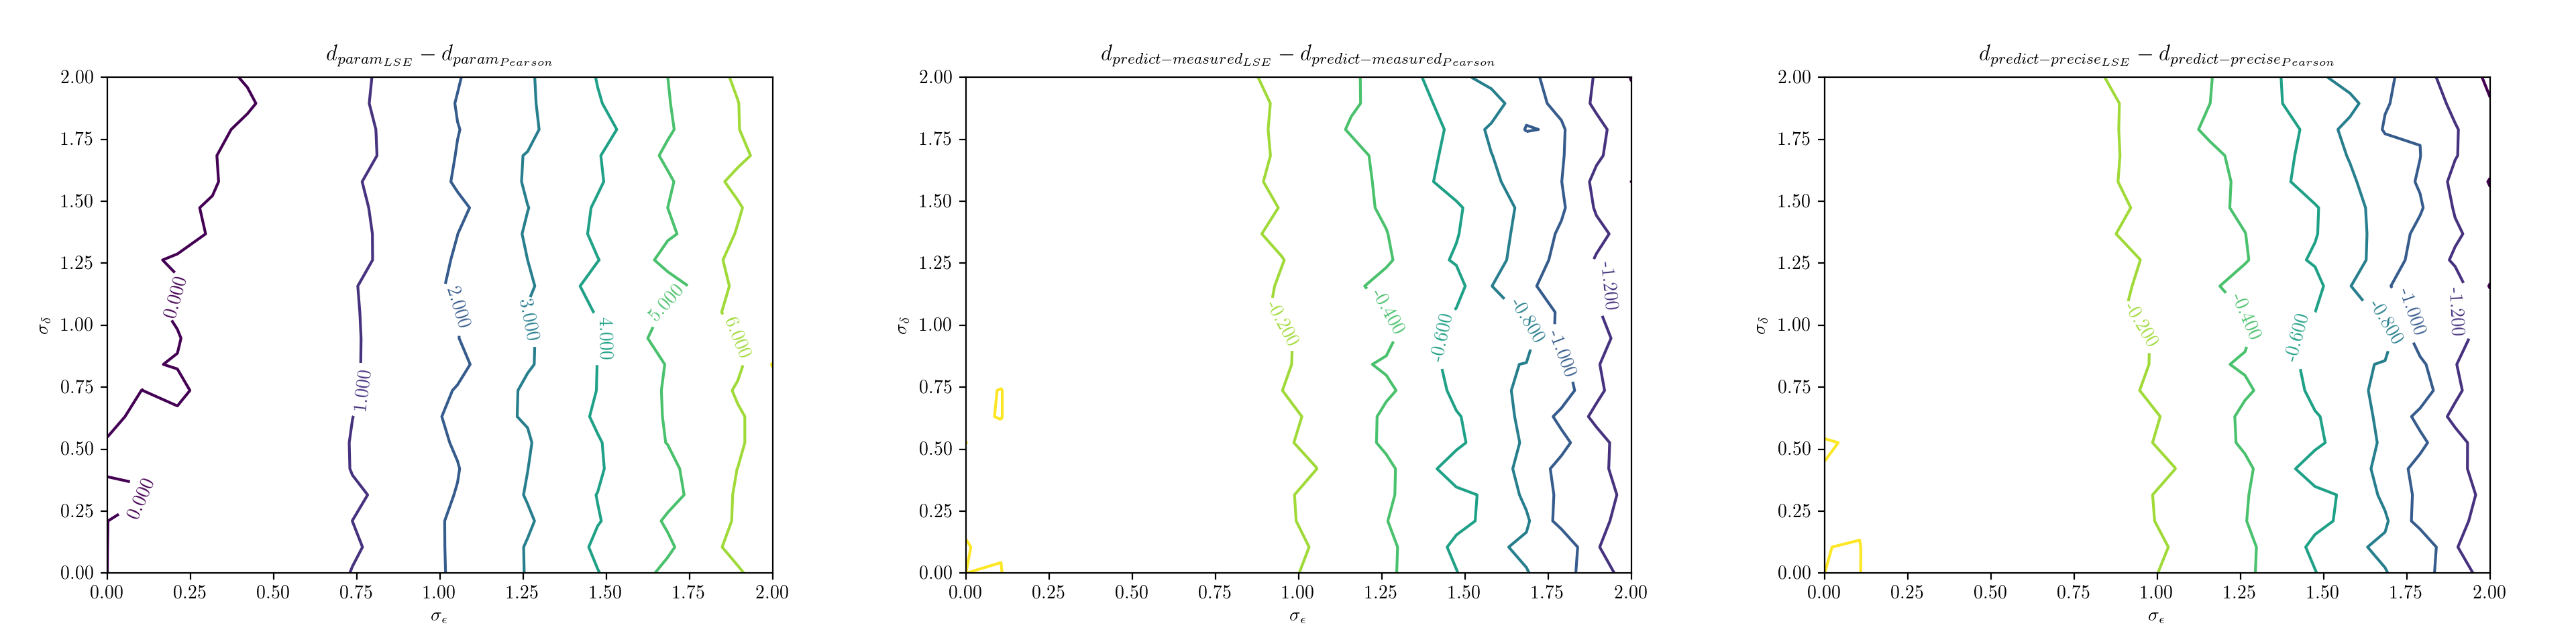
\includegraphics[width=.9\linewidth]{fig/beta-5.png}
  \caption{$ \beta = 5 $}
\end{figure}

\begin{figure}[h!]
  \centering
  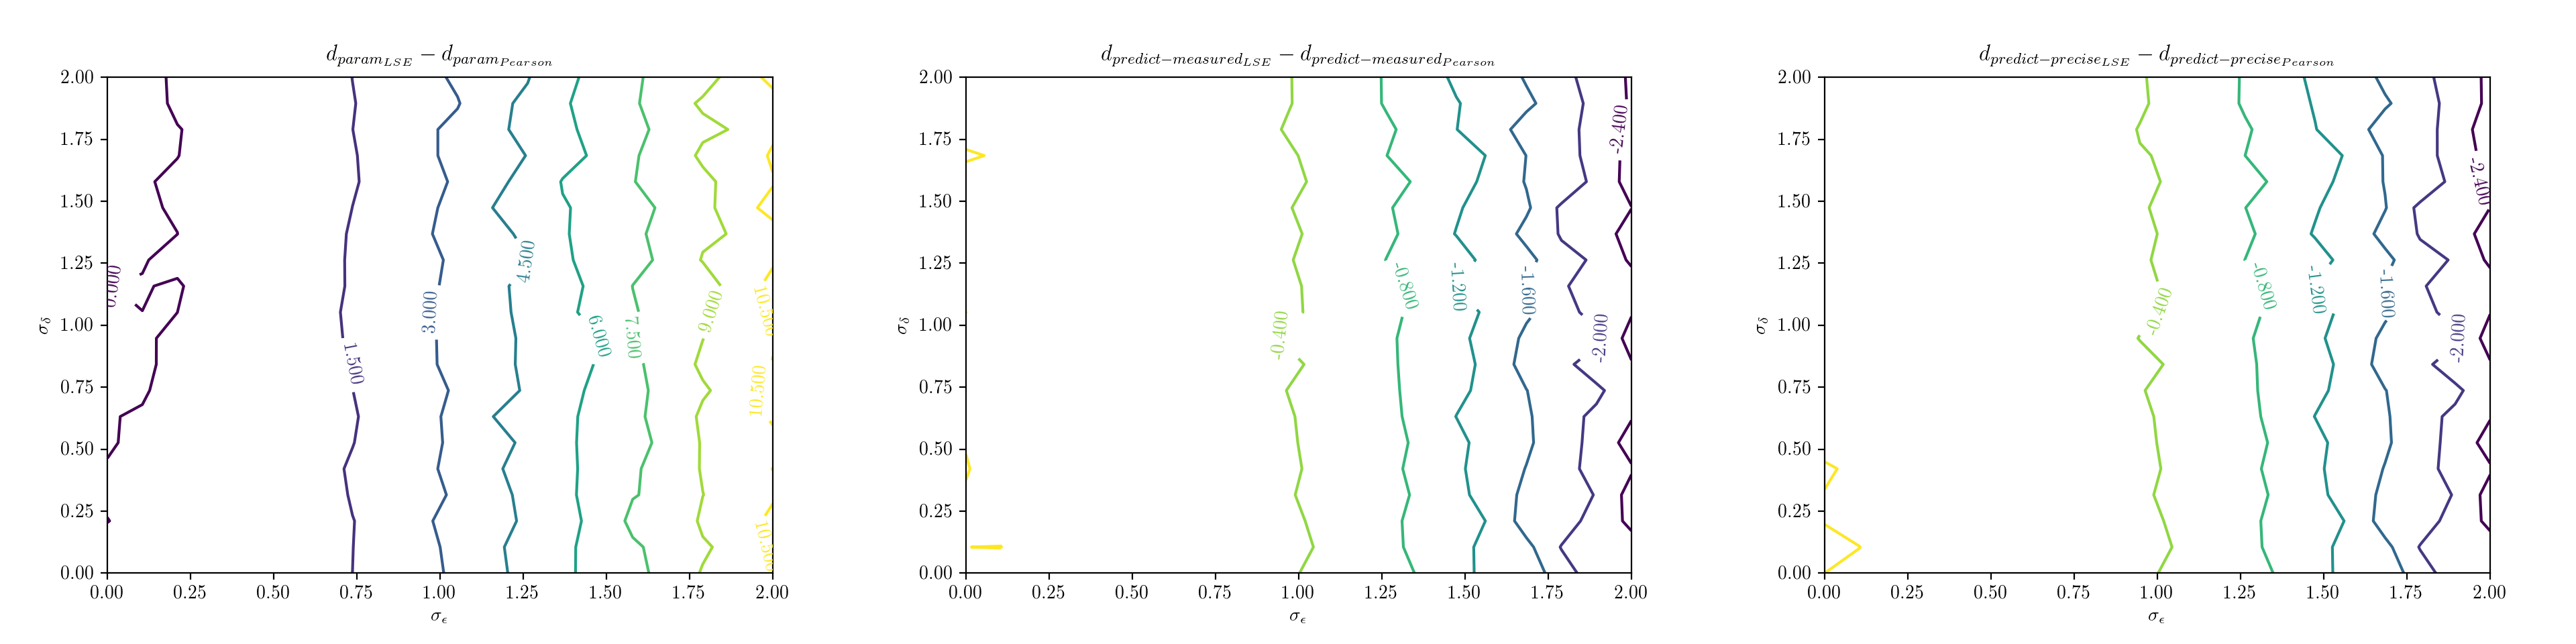
\includegraphics[width=.9\linewidth]{fig/beta-8.png}
  \caption{$ \beta = 8 $}
\end{figure}

\end{document}
